\documentclass{beamer}

\mode<presentation>
{
	\usetheme{CambridgeUS}
	\setbeamercovered{transparent}
}
\usepackage[spanish]{babel}
\usepackage[latin1]{inputenc}
\usepackage{color}
\usepackage{hyperref}
\usepackage{multicol}
\usepackage{algorithm,algorithmic}

\title[\textbf{ICI 4242 - Aut\'omatas y compiladores}]{\textbf{ICI 4242 - Aut\'omatas y compiladores}}

\subtitle{Aut\'omatas finitos}

\author[Rodrigo Olivares]
{
	Rodrigo Olivares \\
	\vspace{0.5mm}
	Mg. en Ingenier\'ia Inform\'atica \\
	\vspace{0.5mm}
	\texttt{\normalsize rodrigo.olivares@uv.cl}
}

\institute[PUCV]

\date{1er Semestre} 

\subject{Aut\'omatas finitos}

%\AtBeginSection
%{
%	\begin{frame}<beamer>
%	\frametitle{Contenido}
%	\tableofcontents[currentsection,currentsubsection]
%	\end{frame}
%}
%
%\AtBeginSubsection
%{
%	\begin{frame}<beamer>
%	\frametitle{Contenido}
%	\tableofcontents[currentsection,currentsubsection]
%	\end{frame}
%}

%\beamerdefaultoverlayspecification{<+->}

\begin{document}

	\begin{frame}
		\titlepage
	\end{frame}

	\begin{frame}
		\frametitle{Contenido}
		\tableofcontents%[pausesections]
	\end{frame}

	\section{Introducci\'on}

		\subsection{Modelado de sistemas discretos}

		\begin{frame}
			\frametitle{Introducci\'on}
			\framesubtitle{Modelado de sistemas discretos}

			\begin{block}{Abstracci\'on}
			    \emph{La realidad es continua}, por lo tanto los sistemas discretos son una abstracci\'on del mundo real. La noci\'on m\'as b\'asica de los modelos de eventos discretos es la de \textbf{estado}. 
			\end{block}
			\begin{block}{Estado}
			    Un estado es una situaci\'on en la que se permanece un cierto lapso de tiempo. 
			\end{block}
		\end{frame}

		\begin{frame}
			\frametitle{Introducci\'on}
			\framesubtitle{Modelado de sistemas discretos}

			\begin{exampleblock}{Ejemplo}
			    Un ejemplo de la vida real es el de los ``estados civiles", que puede estar una persona: soltera, casada, viuda, divorciada, etc. De uno de estos estados se puede pasar a otro al ocurrir un evento o acci\'on. As\'i, por ejemplo, del estado ``soltero", se puede pasar al estado ``casado", al ocurrir el evento ``boda". Similarmente, se puede pasar de ``casado", a ``divorciado", mediante el evento ``divorcio". 
			\end{exampleblock}
		\end{frame}

		\begin{frame}
			\frametitle{Introducci\'on}
			\framesubtitle{Modelado de sistemas discretos}

			\begin{center}
			    \fbox{\fbox{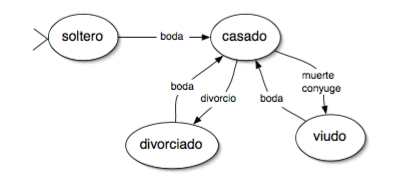
\includegraphics[scale=.75]{images/e1.png}}}
			\end{center}
		\end{frame}

		\begin{frame}
			\frametitle{Introducci\'on}
			\framesubtitle{Modelado de sistemas discretos}

            \begin{block}{Estados finales}
                El prop\'osito de algunos modelos de estados y eventos es el de reconocer secuencias de eventos ``buenas", de manera que se les pueda diferencias de las secuencias ``malas".
            \end{block}
		\end{frame}

		\begin{frame}
			\frametitle{Introducci\'on}
			\framesubtitle{Modelado de sistemas discretos}

            \begin{exampleblock}{Cobro aut\'omatico}
                El dispensador acepta monedas de valor 1, 2 y 5, y el precio de cada lata es de 5. Vamos a considerar que el evento llamado ``1" es la introducci\'on de una moneda de valor 1 en la m\'aquina, el evento ``2" para la moneda de valor 2, etc.
            \end{exampleblock}
            \begin{exampleblock}{}
                La primera cuesti\'on que hay que resolver para dise\~nar nuestro modelo es decidir c\'omo son los estados. Una buena idea ser\'ia que cada estado recordara lo que se lleva acumulado hasta el momento. El estado inicial, desde luego, recordar\'ia que se lleva acumulado 0. 
            \end{exampleblock}
		\end{frame}

		\begin{frame}
			\frametitle{Introducci\'on}
			\framesubtitle{Modelado de sistemas discretos}

			\begin{center}
			    \fbox{\fbox{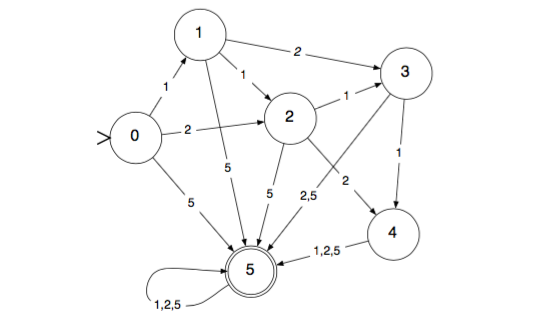
\includegraphics[scale=.5]{images/e2.png}}}
			\end{center}
		\end{frame}

	\section{Aut\'omatas finitos}

        \subsection{M\'aquinas de estados finitos}

        \begin{frame}
			\frametitle{Aut\'omatas finitos}
			\framesubtitle{M\'aquinas de estados finitos}

            \begin{block}{Evento a Transici\'on}
                A partir de ahora vamos a considerar modelos de estados y eventos un poco m\'as abstractos que los que hemos visto antes. Retomemos el ejemplo de la m\'aquina dispensadora. En ese modelo es posible reconocer secuencias de eventos ``aceptables", como la secuencia de monedas $2, 2, 1$ con respecto a secuencias no aceptables, como $1, 1, 1$. A partir de ahora los nombres de los eventos van a estar formados por un caracter, y les llamaremos \textbf{transiciones} en vez de ``eventos".
            \end{block}
		\end{frame}

        \begin{frame}
			\frametitle{Aut\'omatas finitos}
			\framesubtitle{M\'aquinas de estados finitos}

            \begin{block}{Transici\'on}
                De este modo, por ejemplo, en vez de un evento ``meter 1", vamos a tener una transici\'on con el caracter ``1". Desde luego, la elecci\'on de qu\'e caracter tomar como nombre de la transici\'on es una decisi\'on arbitraria.
            \end{block}
            \begin{block}{Secuencia de transici\'on}
                Las secuencias de transiciones van a representarse por concatenaciones de caracteres, esto es, por palabras. As\'i, en el ejemplo de la m\'aquina dispensadora la palabra ``1121", representa la secuencia de eventos ``meter 1", ``meter 1", ``meter 2", ``meter 1".
            \end{block}
		\end{frame}

        \begin{frame}
			\frametitle{Aut\'omatas finitos}
			\framesubtitle{M\'aquinas de estados finitos}

            \begin{block}{M\'aquina abstracta}
                \begin{multicols}{2}
                    Desde el punto de vista abstracto las m\'aquinas pueden ser visualizadas como dispositivos con los siguientes componentes:
                    \begin{itemize}
                       \item Una cinta de entrada;
                       \item Una cabeza de lectura (y eventualmente escritura);
                       \item Un control.
                    \end{itemize}
                    \begin{center}
			            \fbox{\fbox{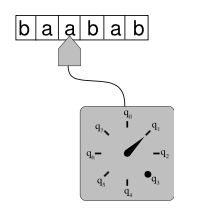
\includegraphics[scale=.65]{images/e3.png}}}
			        \end{center}
                \end{multicols}
            \end{block}
		\end{frame}

        \subsection{Definici\'on formal AFD}

        \begin{frame}
			\frametitle{Aut\'omatas finitos}
			\framesubtitle{Definici\'on formal AFD}

            \begin{block}{Definici\'on}
                Al describir una m\'aquina de estados finitos en particular, debemos incluir las informaciones que var\'ian de un aut\'omata a otro; es decir, no tiene sentido incluir descripciones generales aplicables a todo aut\'omata. Estas informaciones son exactamente las que aparecen en un diagrama de estados y transiciones.
            \end{block}
		\end{frame}

        \begin{frame}
			\frametitle{Aut\'omatas finitos}
			\framesubtitle{Definici\'on formal AFD}

            \begin{block}{Definici\'on matem\'atica o formal}
                 Un \textbf{Aut\'omata Finito Determinista} \emph{M} es una qu\'intupla ($Q$, $\Sigma$, $\delta$, $q_{0}$, $F$), donde:
                \begin{itemize}
                    \item[] $Q$: es un conjunto de identificadores (s\'imbolos) de estados;
                    \item[] $\Sigma$: es el alfabeto de entrada;
                    \item[] $\delta$: $Q \times \Sigma \rightarrow Q$ es la funci\'on de transici\'on, que a partir de un estado y un s\'imbolo del alfabeto obtiene un nuevo estado.
                    \item[] $q_{0} \in Q$: es el estado inicial
                    \item[] $F \subset Q$: es un conjunto de estados finales;
                \end{itemize}
            \end{block}
		\end{frame}

        \begin{frame}
			\frametitle{Aut\'omatas finitos}
			\framesubtitle{Definici\'on formal AFD}

            \begin{block}{Definici\'on matem\'atica o formal}
               La funci\'on de transici\'on indica a qu\'e estado se va a pasar sabiendo cu\'al es el estado actual y el s\'imbolo que se est\'a leyendo. Es importante notar que $\delta$ es una \textbf{funci\'on} y no simplemente una relaci\'on; esto implica que para un estado y un s\'imbolo del alfabeto dados, habr\'a un y s\'olo un estado siguiente. Esta caracter\'istica se denomina \emph{determinismo} y la definici\'on dada corresponde a los \textbf{aut\'omatas finitos determin\'istas} o AFD.
            \end{block}
		\end{frame}

        \begin{frame}
			\frametitle{Aut\'omatas finitos}
			\framesubtitle{Definici\'on formal AFD}

            \begin{exampleblock}{Ejemplo AFD}
               Si consideramos el siguiente aut\'omata:
               \begin{center}
			       \fbox{\fbox{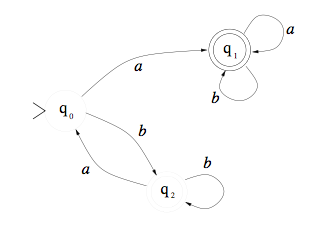
\includegraphics[scale=.5]{images/afd1.png}}}
			   \end{center}
            \end{exampleblock}
		\end{frame}
		
        \begin{frame}
			\frametitle{Aut\'omatas finitos}
			\framesubtitle{Definici\'on formal AFD}

            \begin{exampleblock}{Ejemplo AFD}
               Puede ser expresado formalmente como: $M = (Q, \Sigma, \delta, q_{0}, F)$, donde:
               \begin{itemize}
                   \item[] $Q = \{q_{0},q_{1},q_{2}\}$
                   \item[] $\Sigma = \{a,b\}$
                   \item[] $\delta =  \{((q_{0}, a), q_{1}), ((q_{0}, b), q_{2}), ((q_{1}, a), q_{1}), ((q_{1}, b), q_{1}), ((q_{2}, a), q_{0}),$ $ ((q_{2}, b), q_{2})\}$
                   \item[] $F = \{q_{1},q_{2}\}$
               \end{itemize}
            \end{exampleblock}
		\end{frame}

        \begin{frame}
			\frametitle{Aut\'omatas finitos}
			\framesubtitle{Definici\'on formal AFD}

            \begin{exampleblock}{Ejemplo AFD}
               La funci\'on de transici\'on $\delta$ puede ser expresada mediante una tabla como la siguiente, para este ejemplo:
               
               \begin{center}
                   \begin{tabular}{c|ccc|} 
                   \cline{2-4}
                       & $q$ & $\sigma$ & $\delta(q,\sigma)$ \\ 
                   \cline{2-4}
                       $\rightarrow$ & $q_{0}$ & a & $q_{1}$ \\
                       $\rightarrow$ & $q_{0}$ & b & $q_{2}$ \\
                       \# & $q_{1}$ & a & $q_{1}$ \\
                       \# & $q_{1}$ & b & $q_{1}$ \\
                       \# & $q_{2}$ & a & $q_{0}$ \\
                       \# & $q_{2}$ & b & $q_{2}$ \\
                   \cline{2-4}
                   \end{tabular}
               \end{center}
            \end{exampleblock}
		\end{frame}

        \begin{frame}
			\frametitle{Aut\'omatas finitos}
			\framesubtitle{Definici\'on formal AFD}

            \begin{exampleblock}{Ejercicios AFDs}
               Construya un aut\'omata finito para cada uno de los siguientes lenguajes (representaci\'on gr\'afica y formal):
               \begin{itemize}
                   \item[] $L_{1} = \{(ab)^{n} | n > 1\}$
                   \item[] $L_{2} = \{a^{n}b^{m} | n \geq 2 \wedge m \geq 3\}$
               \end{itemize}
            \end{exampleblock}
		\end{frame}

        \subsection{Definici\'on formal AFND}

        \begin{frame}
			\frametitle{Aut\'omatas finitos}
			\framesubtitle{Definici\'on formal AFND}

            \begin{block}{Definici\'on}
                Un \emph{aut\'omata finito no determinista} (AFND) es un aut\'omata finito que, a diferencia de los aut\'omatas finitos deterministas, posee al menos un estado $q_{i} \in Q$, tal que para un s\'imbolo $a \in \Sigma$ del alfabeto, existe m\'as de una transici\'on $\delta(q_{i},a)$ posible.
            \end{block}
		\end{frame}

        \begin{frame}
			\frametitle{Aut\'omatas finitos}
			\framesubtitle{Definici\'on formal AFND}

            \begin{block}{Definici\'on}
                En un AFND puede darse cualquiera de estos dos casos:
                \begin{itemize}
                    \item[$\rightarrow$] Que existan transiciones del tipo $\delta(q_{i},a)=q_{j}$ y $\delta(q_{i},a)=q_{k}$, siendo $q_{j} \neq q_{k}$;
                    \item[$\rightarrow$] Que existan transiciones del tipo $\delta(q_{i},\lambda)$, siendo $q_{i}$ un estado \textbf{no-final}, o bien un estado final pero con transiciones hacia otros estados.
                \end{itemize}
            \end{block}
		\end{frame}

        \begin{frame}
			\frametitle{Aut\'omatas finitos}
			\framesubtitle{Definici\'on formal AFND}

            \begin{block}{Definici\'on matem\'atica o formal}
                 Un \textbf{Aut\'omata Finito No Determinista} \emph{M} es una qu\'intupla ($Q$, $\Sigma$, $\delta$, $q_{0}$, $F$), donde:
                \begin{itemize}
                    \item[] $Q$: es un conjunto de identificadores (s\'imbolos) de estados;
                    \item[] $\Sigma$: es el alfabeto de entrada;
                    \item[] $\delta$: $Q \times \Sigma \rightarrow \mathcal{P}(Q)$ (conjunto potencia) es la funci\'on de transici\'on.
                    \item[] $q_{0} \in Q$: es el estado inicial
                    \item[] $F \subset Q$: es un conjunto de estados finales;
                \end{itemize}
            \end{block}
		\end{frame}

        \begin{frame}
			\frametitle{Aut\'omatas finitos}
			\framesubtitle{Definici\'on formal AFND}

            \begin{exampleblock}{Ejemplo AFND}
               Puede ser expresado formalmente como: $M = (Q, \Sigma, \delta, q_{0}, F)$, donde:
               \begin{itemize}
                   \item[] $Q = \{q_{0},q_{1},q_{2}\}$
                   \item[] $\Sigma = \{0,1\}$
                   \item[] $\delta =  \{((q_{0}, 0),q_{0}),((q_{1}, 0),q_{0}),((q_{2}, 0),q_{2}),((q_{0}, 1),q_{0}),((q_{0}, 1),q_{1}),$ $((q_{1}, 1),q_{2}),((q_{2}, 1), q_{1})\}$
                   \item[] $F = \{q_{1}\}$
               \end{itemize}
            \end{exampleblock}
		\end{frame}

        \begin{frame}
			\frametitle{Aut\'omatas finitos}
			\framesubtitle{Definici\'on formal AFND}

            \begin{exampleblock}{Ejemplo AFND}
               Definir la funci\'on de transici\'on $\delta$:
               
               \begin{center}
                   \begin{tabular}{c|ccc|} 
                   \cline{2-4}
                       & $q$ & $\sigma$ & $\delta(q,\sigma)$ \\ 
                   \cline{2-4}
                       & & & \\
                       & & & \\
                       & & & \\
                       & & & \\
                       & & & \\
                       & & & \\
                       & & & \\
                   \cline{2-4}
                   \end{tabular}
               \end{center}
            \end{exampleblock}
		\end{frame}

        \begin{frame}
			\frametitle{Aut\'omatas finitos}
			\framesubtitle{Definici\'on formal AFND}

            \begin{exampleblock}{Ejemplo AFND - Soluci\'on}
               Definir la funci\'on de transici\'on $\delta$:
               
               \begin{center}
                   \begin{tabular}{c|ccc|} 
                   \cline{2-4}
                       & $q$ & $\sigma$ & $\delta(q,\sigma)$ \\ 
                   \cline{2-4}
                       $\rightarrow$
                       & $q_{0}$ & 0 & $q_{0}$ \\
                       & $q_{0}$ & 1 & $q_{0}$ \\
                       & $q_{0}$ & 1 & $q_{1}$ \\
                       \# 
                       & $q_{1}$ & 0 & $q_{0}$ \\
                       & $q_{1}$ & 1 & $q_{2}$ \\
                       & $q_{2}$ & 0 & $q_{2}$ \\
                       & $q_{2}$ & 1 & $q_{1}$ \\
                   \cline{2-4}
                   \end{tabular}
               \end{center}
            \end{exampleblock}
		\end{frame}

        \begin{frame}
			\frametitle{Aut\'omatas finitos}
			\framesubtitle{Definici\'on formal AFND}

            \begin{exampleblock}{Ejemplo AFND - Soluci\'on}
               \begin{center}
			       \fbox{\fbox{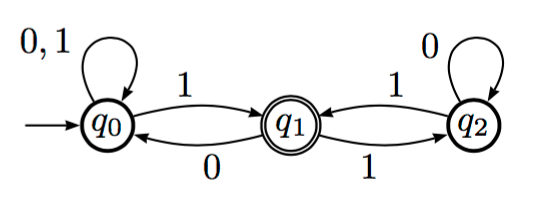
\includegraphics[scale=.5]{images/afnd1.png}}}
			   \end{center}
            \end{exampleblock}
		\end{frame}

        \subsection{Definici\'on formal $\lambda$-AFND}

        \begin{frame}
			\frametitle{Aut\'omatas finitos}
			\framesubtitle{Definici\'on formal $\lambda$-AFND}

            \begin{block}{Definici\'on}
                Estas transiciones permiten al aut\'omata cambiar de estado \textbf{sin procesar/consumir ning\'un s\'imbolo de entrada}.
            \end{block}
		\end{frame}

        \begin{frame}
			\frametitle{Aut\'omatas finitos}
			\framesubtitle{Definici\'on formal $\lambda$-AFND}

            \begin{block}{Definici\'on matem\'atica o formal}
                \textbf{Aut\'omata Finito No Determinista con} $\lambda$-\textbf{transiciones} \emph{M} es una qu\'intupla ($Q$, $\Sigma$, $\delta$, $q_{0}$, $F$), donde:
                \begin{itemize}
                    \item[] $Q$: es un conjunto de identificadores (s\'imbolos) de estados;
                    \item[] $\Sigma$: es el alfabeto de entrada;
                    \item[] $\delta$: $Q \times (\Sigma \cup \lambda) \rightarrow \mathcal{P}(Q)$ (conjunto potencia) es la funci\'on de transici\'on.
                    \item[] $q_{0} \in Q$: es el estado inicial
                    \item[] $F \subset Q$: es un conjunto de estados finales;
                \end{itemize}
            \end{block}
		\end{frame}

        \begin{frame}
			\frametitle{Aut\'omatas finitos}
			\framesubtitle{Definici\'on formal $\lambda$-AFND}

            \begin{exampleblock}{Ejemplo $\lambda$-AFND}
               Puede ser expresado formalmente como: $M = (Q, \Sigma, \delta, q_{0}, F)$, donde:
               \begin{itemize}
                   \item[] $Q = \{q_{0},q_{1},q_{2}\}$
                   \item[] $\Sigma = \{0,1\}$
                   \item[] $\delta =  \{((q_{0}, 0),q_{0}),((q_{1}, 0),q_{0}),((q_{2}, 0),q_{2}),((q_{0}, 1),q_{0}),((q_{0}, 1),q_{1}),$ $((q_{1}, 1),q_{2}),((q_{2}, \lambda), q_{1})\}$
                   \item[] $F = \{q_{1}\}$
               \end{itemize}
            \end{exampleblock}
		\end{frame}

        \begin{frame}
			\frametitle{Aut\'omatas finitos}
			\framesubtitle{Definici\'on formal $\lambda$-AFND}

            \begin{exampleblock}{Ejemplo $\lambda$-AFND}
               Definir la funci\'on de transici\'on $\delta$:
               
               \begin{center}
                   \begin{tabular}{c|ccc|} 
                   \cline{2-4}
                       & $q$ & $\sigma$ & $\delta(q,\sigma)$ \\ 
                   \cline{2-4}
                       & & & \\
                       & & & \\
                       & & & \\
                       & & & \\
                       & & & \\
                       & & & \\
                       & & & \\
                   \cline{2-4}
                   \end{tabular}
               \end{center}
            \end{exampleblock}
		\end{frame}

        \begin{frame}
			\frametitle{Aut\'omatas finitos}
			\framesubtitle{Definici\'on formal $\lambda$-AFND}

            \begin{exampleblock}{Ejemplo $\lambda$-AFND - Soluci\'on}
               Definir la funci\'on de transici\'on $\delta$:
               
               \begin{center}
                   \begin{tabular}{c|ccc|} 
                   \cline{2-4}
                       & $q$ & $\sigma$ & $\delta(q,\sigma)$ \\ 
                   \cline{2-4}
                       $\rightarrow$
                       & $q_{0}$ & 0 & $q_{0}$ \\
                       & $q_{0}$ & 1 & $q_{0}$ \\
                       & $q_{0}$ & 1 & $q_{1}$ \\
                       \# 
                       & $q_{1}$ & 0 & $q_{0}$ \\
                       & $q_{1}$ & 1 & $q_{2}$ \\
                       & $q_{2}$ & 0 & $q_{2}$ \\
                       & $q_{2}$ & $\lambda$ & $q_{1}$ \\
                   \cline{2-4}
                   \end{tabular}
               \end{center}
            \end{exampleblock}
		\end{frame}

        \begin{frame}
			\frametitle{Aut\'omatas finitos}
			\framesubtitle{Definici\'on formal $\lambda$-AFND}

            \begin{exampleblock}{Ejemplo $\lambda$-AFND - Soluci\'on}
               \begin{center}
			       \fbox{\fbox{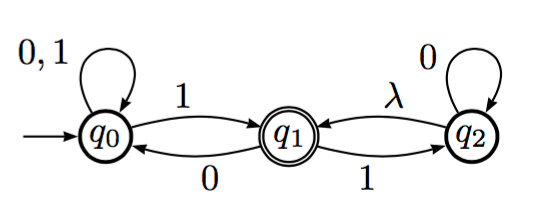
\includegraphics[scale=.5]{images/afndl1.png}}}
			   \end{center}
            \end{exampleblock}
		\end{frame}

    \section{Conversiones}

        \subsection{AFND a AFD}
       
        \begin{frame}
			\frametitle{Conversiones}
			\framesubtitle{AFND a AFD}

            \begin{block}{AFND a AFD}
               Existe una equivalencia entre los AFD y AFND, de forma que un aut\'omata \textbf{M} es equivalente a un aut\'omata \textbf{M'}, \emph{ssi} $L(M) = L(M')$. Este procedimiento, es llamado \textbf{construcci\'on de subconjuntos}.
            \end{block}
		\end{frame}

        \begin{frame}
			\frametitle{Conversiones}
			\framesubtitle{AFND a AFD}

            \begin{block}{Algoritmo}
               \begin{enumerate}
                   \item[1.-] Construir una tabla con columnas, una por cada $\sigma \in \Sigma$.
                   \item[2.-] En la primera fila, escribir $\{q_{0}\}$ y en la columna $\sigma_{i}$ escribir $\delta(\{q_{0}\},\sigma_{i})$, es decir, todos los estados a los que puedo llegar desde $q_{0}$ con entrada $\sigma_{i}$.
                   \item[3.-] Copiar las casillas de la fila anterior como principio de nuevas filas.
                   \item[4.-] Para cada fila \emph{R} pendiente, rellenar la fila \emph{R} escribiendo en cada columna $\sigma_{i}$, $\delta(R,\sigma_{i})$, es decir, todos los estados a los que puedo llegar desde alg\'un estado de \emph{R} con entrada $\sigma_{i}$.
                   \item[5.-] Repetir los pasos 3 y 4 hasta que no queden filas por rellenar.
               \end{enumerate}
            \end{block}
		\end{frame}

        \begin{frame}
			\frametitle{Conversiones}
			\framesubtitle{AFND a AFD}

            \begin{exampleblock}{Ejemplo}
               Seg\'un el siguiente AFND, construya el AFD equivalente.
               \begin{center}
			       \fbox{\fbox{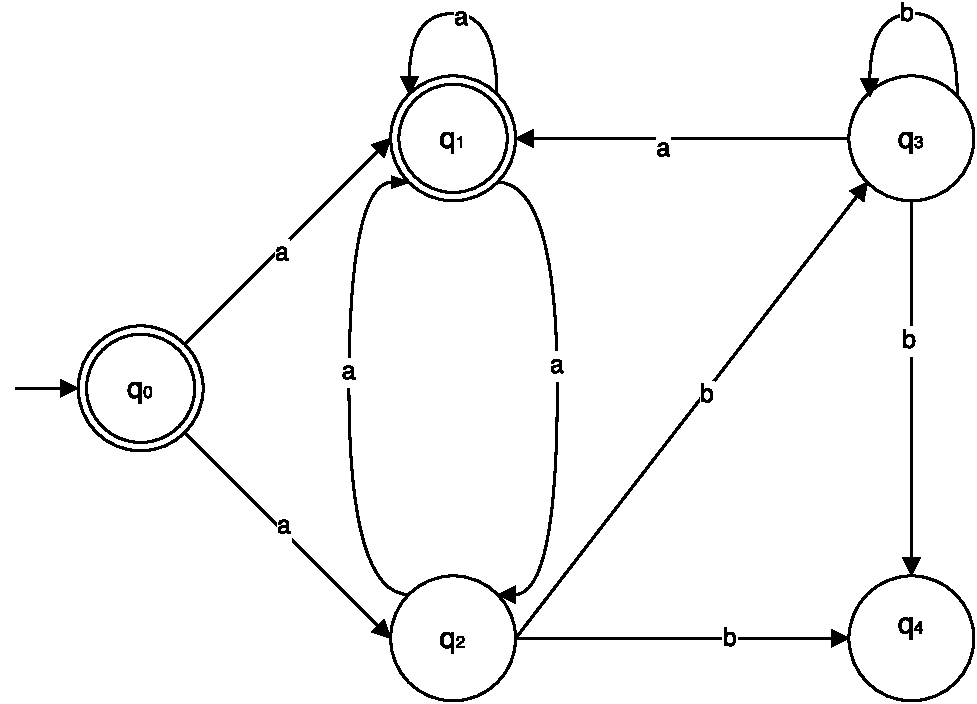
\includegraphics[scale=.35]{images/conv-afnd-1.pdf}}}
			   \end{center}
            \end{exampleblock}
		\end{frame}
		
        \begin{frame}
			\frametitle{Conversiones}
			\framesubtitle{AFND a AFD}

            \begin{exampleblock}{Ejemplo - Soluci\'on}
               \begin{table}
                   \begin{center}
                       \begin{tabular}{c|c|c} 
                           $\{Q\}$ & $a$ & $b$ \\ \hline
                           $\{q_{0}\}$ & $\{q_{1}, q_{2}\}$ & $---$ \\
                           $\{q_{1}, q_{2}\}$ & $\{q_{1}, q_{2}\}$ & $\{q_{3}, q_{4}\}$ \\
                           $\{q_{3}, q_{4}\}$ & $\{q_{1}\}$ & $\{q_{3}, q_{4}\}$ \\
                           $\{q_{1}\}$ & $\{q_{1}, q_{2}\}$ & $---$ \\
                       \end{tabular}
                   \end{center}
               \end{table}
            \end{exampleblock}
		\end{frame}				
		
        \begin{frame}
			\frametitle{Conversiones}
			\framesubtitle{AFND a AFD}

            \begin{exampleblock}{Ejemplo - Soluci\'on (\textbf{renombrando estados})}
               \begin{table}
                   \begin{center}
                       \begin{tabular}{c|c|c|c} 
                           $\{Q\}$ & $a$ & $b$ & $q_{i}'$ \\ \hline
                           $\{q_{0}\}$ & $\{q_{1}, q_{2}\}$ & $---$ & $q_{0}'$\\
                           $\{q_{1}, q_{2}\}$ & $\{q_{1}, q_{2}\}$ & $\{q_{3}, q_{4}\}$ & $q_{2}'$ \\
                           $\{q_{3}, q_{4}\}$ & $\{q_{1}\}$ & $\{q_{3}, q_{4}\}$ & $q_{3}'$ \\
                           $\{q_{1}\}$ & $\{q_{1}, q_{2}\}$ & $---$ & $q_{1}'$\\
                       \end{tabular}
                   \end{center}
               \end{table}
            \end{exampleblock}
		\end{frame}		
		
        \begin{frame}
			\frametitle{Conversiones}
			\framesubtitle{AFND a AFD}

            \begin{exampleblock}{Ejemplo - Soluci\'on (\textbf{renombrando estados})}
               \begin{table}
                   \begin{center}
                       \begin{tabular}{c|c|c} 
                           $\{Q\}$ & $a$ & $b$\\ \hline
                           $\{q_{0}'\}$ & $\{q_{2}'\}$ & $---$ \\
                           $\{q_{2}'\}$ & $\{q_{2}'\}$ & $\{q_{3}'\}$ \\
                           $\{q_{3}'\}$ & $\{q_{1}'\}$ & $\{q_{3}'\}$ \\
                           $\{q_{1}'\}$ & $\{q_{2}'\}$ & $---$ \\
                       \end{tabular}
                   \end{center}
               \end{table}
            \end{exampleblock}
		\end{frame}			
		
        \begin{frame}
			\frametitle{Conversiones}
			\framesubtitle{AFND a AFD}

            \begin{exampleblock}{Ejemplo - Soluci\'on}
               \begin{center}
			       \fbox{\fbox{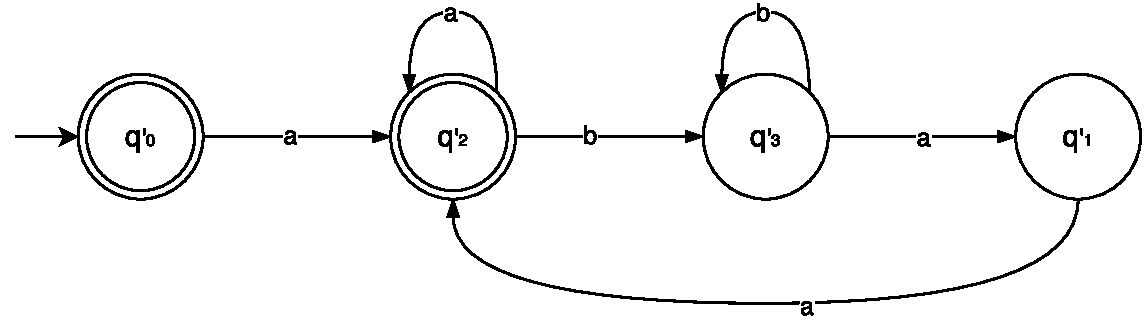
\includegraphics[scale=.35]{images/conv-afnd-1-1.pdf}}}
			       $$G = \cdots $$
			       $$M' = \cdots $$
			       $$L(G) = \{\lambda~|~a^{n+1}~|~(a^{n+1}b^{m+1})aa~/~n \geqslant 0 \wedge m \geqslant 0 \}$$
			       El automata no posee una $\lambda$-transici\'on, sin embargo la cadena vac\'ia es aceptada por el lenguaje.
			   \end{center}
            \end{exampleblock}
		\end{frame}		
		
        \begin{frame}
			\frametitle{Conversiones}
			\framesubtitle{AFND a AFD}

            \begin{exampleblock}{Ejercicio}
               Seg\'un el siguiente AFND, construya el AFD equivalente.
               \begin{center}
			       \fbox{\fbox{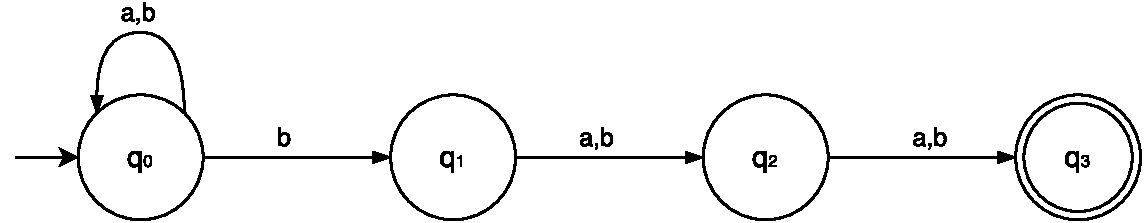
\includegraphics[scale=.45]{images/conv-afnd-2.pdf}}}
			   \end{center}
            \end{exampleblock}
		\end{frame}		
		
        \begin{frame}
			\frametitle{Conversiones}
			\framesubtitle{AFND a AFD}

            \begin{exampleblock}{Ejercicio - Soluci\'on}
               \begin{table}
                   \begin{center}
                       \begin{tabular}{c|c|c|c} 
                           $\{Q\}$ & $a$ & $b$ & $\{q_{i}'\}$ \\ \hline
                           $\{q_{0}\}$ & $\{q_{0}\}$ & $\{q_{0},q_{1}\}$ & $\{q_{0}'\}$ \\
                           $\{q_{0}, q_{1}\}$ & $\{q_{0}, q_{2}\}$ & $\{q_{0}, q_{1}, q_{2}\}$ & $\{q_{1}'\}$ \\
                           $\{q_{0}, q_{2}\}$ & $\{q_{0}, q_{3}\}$ & $\{q_{0}, q_{1}, q_{3}\}$ & $\{q_{2}'\}$ \\
                           $\{q_{0}, q_{1}, q_{2}\}$ & $\{q_{0}, q_{2}, q_{3}\}$ & $\{q_{0}, q_{1}, q_{2}, q_{3}\}$ & $\{q_{3}'\}$ \\
                           $\{q_{0}, q_{3}\}$ & $\{q_{0}\}$ & $\{q_{0},q_{1}\}$ & $\{q_{4}'\}$ \\
                           $\{q_{0}, q_{1}, q_{3}\}$ & $\{q_{0}, q_{2}\}$ & $\{q_{0}, q_{1}, q_{2}\}$ & $\{q_{5}'\}$ \\
                           $\{q_{0}, q_{2}, q_{3}\}$ & $\{q_{0}, q_{3}\}$ & $\{q_{0}, q_{1}, q_{3}\}$ & $\{q_{6}'\}$ \\
                           $\{q_{0}, q_{1}, q_{2}, q_{3}\}$& $\{q_{0}, q_{2}, q_{3}\}$ & $\{q_{0}, q_{1}, q_{2}, q_{3}\}$ & $\{q_{7}'\}$ \\
                       \end{tabular}
                   \end{center}
               \end{table}
            \end{exampleblock}
		\end{frame}				
		
        \begin{frame}
			\frametitle{Conversiones}
			\framesubtitle{AFND a AFD}
           
               \hspace{4cm}\huge{\textquestiondown~Aut\'omata ?}
%               \begin{center}
%			       \fbox{\fbox{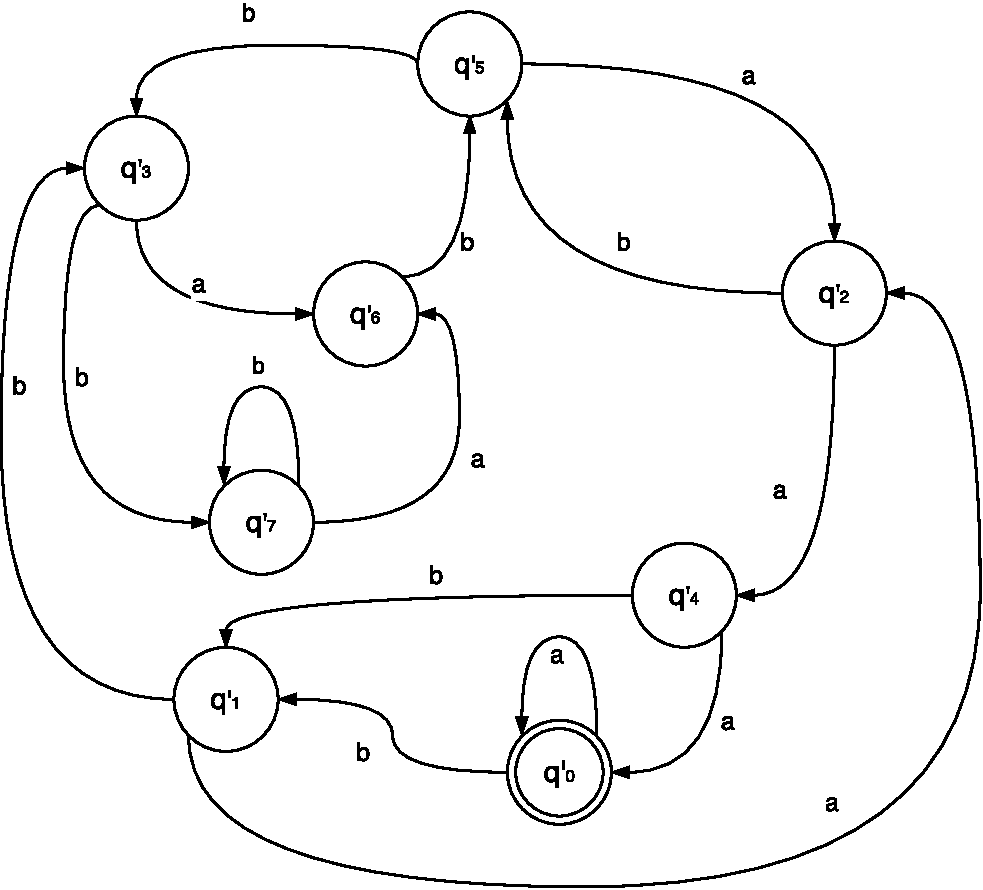
\includegraphics[scale=.4]{images/conv-afnd-2-2.pdf}}}
%			   \end{center}
		\end{frame}	
		
        \subsection{$\lambda$-AFND a AFD}		
		
        \begin{frame}
			\frametitle{Conversiones}
			\framesubtitle{$\lambda$-AFND a AFD}

            \begin{block}{$\lambda$-AFND a AFD}
               Tenemos un AFND $M$ que puede tener $\lambda$-transiciones. Para cada $R \in Q$ definimos $E(R)$, el conjunto de estados alcanzables desde $R$ mediante $\lambda$-transiciones.
            \end{block}
		\end{frame}

        \begin{frame}
			\frametitle{Conversiones}
			\framesubtitle{$\lambda$-AFND a AFD}

            \begin{block}{Algoritmo}
               \begin{enumerate}
                   \item[1.-] Construir una tabla con columnas, una por cada $\sigma \in \Sigma$.
                   \item[2.-] En la primera fila escribir el inicial $I = E(\{q_{0}\})$, es decir, todos los estados a los que puedo llegar desde $q_{0}$ con $\lambda^{*}$.
                   \item[3.-] En la primera fila, en la columna $\sigma_{i}$ escribir $\cup_{r \in I} E(\delta(r,\sigma_{i}))$, es decir, todos los estados a los que puedo llegar desde $I$ con entrada $\sigma_{i}\lambda^{*}$.
                   \item[4.-] Copiar las casillas de la fila anterior como principio de nuevas filas.
                   \item[5.-] Para cada fila $R$ pendiente, rellenar la fila $R$ escribiendo en cada columna $\sigma_{i}$, $\cup_{r \in R} E(\delta(r,\sigma_{i}))$, es decir, todos los estados a los que puedo llegar desde alg\'un estado de $R$ con entrada $\sigma_{i}\lambda^{*}$.
                   \item[6.-] Repetir los pasos 4 y 5 hasta que no queden filas por rellenar.
               \end{enumerate}
            \end{block}
		\end{frame}

        \begin{frame}
			\frametitle{Conversiones}
			\framesubtitle{$\lambda$-AFND a AFD}

            \begin{exampleblock}{Ejemplo}
               Seg\'un el siguiente $\lambda$-AFND, construya el AFD equivalente.
               \begin{center}
			       \fbox{\fbox{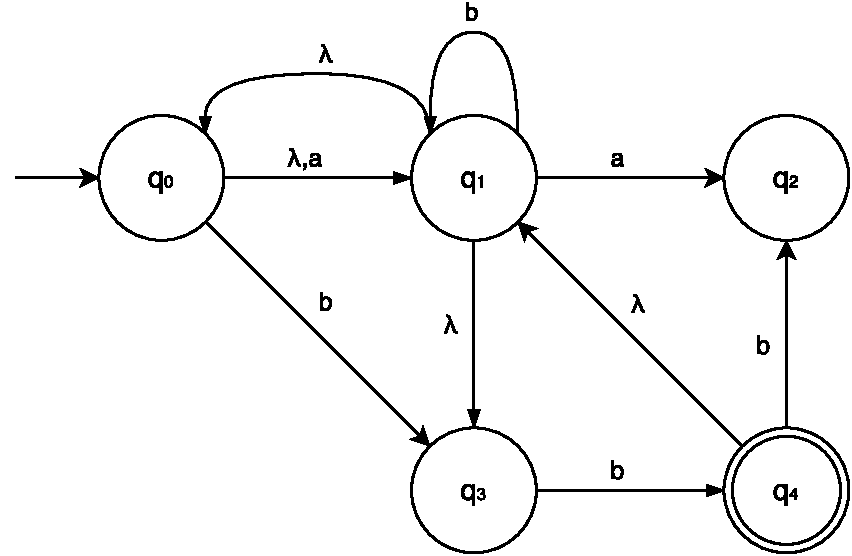
\includegraphics[scale=.4]{images/conv-l-afnd-1.pdf}}}
			   \end{center}
            \end{exampleblock}
		\end{frame}

        \begin{frame}
			\frametitle{Conversiones}
			\framesubtitle{$\lambda$-AFND a AFD}

            \begin{exampleblock}{Ejemplo - Soluci\'on}
               \begin{table}
                   \begin{center}
                    {\tiny
                       \begin{tabular}{l|c|lc} 
                           \multicolumn{1}{c|}{$E(\{q_{i}\})$} & \multicolumn{1}{c}{$a$} & \multicolumn{1}{|c}{$b$} & \multicolumn{1}{|c}{$q_{i}'$} \\ \hline
                           $A=\{q_{0}\} \cup \{q_{0},q_{1},q_{3}\}$ & $B=\{q_{1},q_{2}\} \cup \{q_{0},q_{1},q_{3}\}$ & $C=\{q_{1},q_{3},q_{4}\} \cup \{q_{0},q_{1},q_{3}\}$ & $q_{0}'$ \\
                           $B=\{q_{1},q_{2}\} \cup \{q_{0},q_{1},q_{3}\}$ & $B=\{q_{1},q_{2}\} \cup \{q_{0},q_{1},q_{3}\}$ & $C=\{q_{1},q_{3},q_{4}\} \cup \{q_{0},q_{1},q_{3}\}$ & $q_{1}'$ \\
                           $C=\{q_{1},q_{3},q_{4}\} \cup \{q_{0},q_{1},q_{3}\}$ & $B=\{q_{1},q_{2}\} \cup \{q_{0},q_{1},q_{3}\}$ & $D=\{q_{1},q_{2},q_{3},q_{4}\} \cup \{q_{0},q_{1},q_{3}\}$ & $q_{2}'$ \\
                           $D=\{q_{1},q_{2},q_{3},q_{4}\} \cup \{q_{0},q_{1},q_{3}\}$ & $B=\{q_{1},q_{2}\} \cup \{q_{0},q_{1},q_{3}\}$ & $D=\{q_{1},q_{2},q_{3},q_{4}\} \cup \{q_{0},q_{1},q_{3}\}$ & $q_{3}'$ \\
                       \end{tabular}}
                   \end{center}
               \end{table}
            \end{exampleblock}
		\end{frame}		

        \begin{frame}
			\frametitle{Conversiones}
			\framesubtitle{$\lambda$-AFND a AFD}

            \begin{exampleblock}{Ejemplo - Soluci\'on (\textbf{renombrando conjunto de estados})}
               \begin{table}
                   \begin{center}
                       \begin{tabular}{lc|c|c} 
                           & $E(\{q_{i}\})$ & $a$ & $b$ \\ \hline
                           $\rightarrow$ & $q_{0}'$ & $q_{1}'$ & $q_{2}'$ \\
                           & $q_{1}'$ & $q_{1}'$ & $q_{2}'$ \\
                           \# & $q_{2}'$ & $q_{1}'$ & $q_{3}'$ \\
                           \# & $q_{3}'$ & $q_{1}'$ & $q_{3}'$ \\
                       \end{tabular}
                   \end{center}
               \end{table}
            \end{exampleblock}
		\end{frame}		

        \begin{frame}
			\frametitle{Conversiones}
			\framesubtitle{$\lambda$-AFND a AFD}

            \begin{exampleblock}{Ejemplo}
               Seg\'un el siguiente $\lambda$-AFND, construya el AFD equivalente.
               \begin{center}
			       \fbox{\fbox{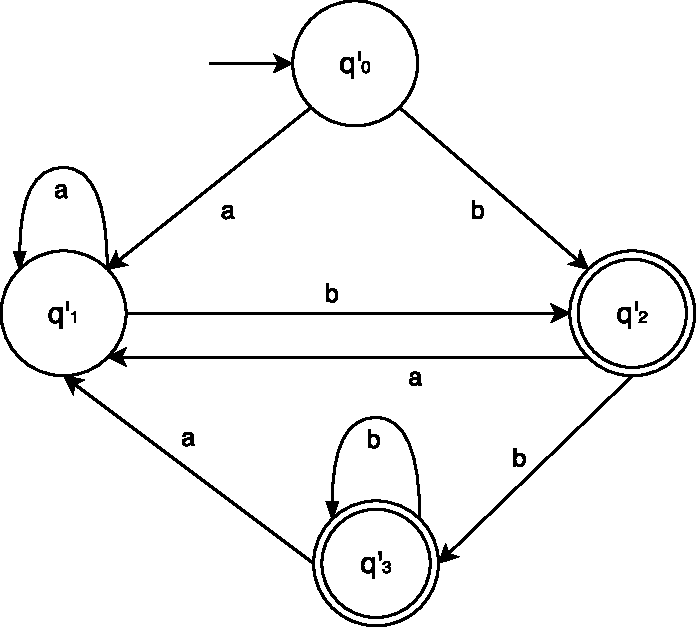
\includegraphics[scale=.4]{images/conv-l-afnd-1-2.pdf}}}
			   \end{center}
            \end{exampleblock}
		\end{frame}	

        \begin{frame}
			\frametitle{Conversiones}
			\framesubtitle{$\lambda$-AFND a AFD}

            \begin{exampleblock}{Ejercicio}
               Seg\'un el siguiente $\lambda$-AFND, construya el AFD equivalente.
               \begin{center}
			       \fbox{\fbox{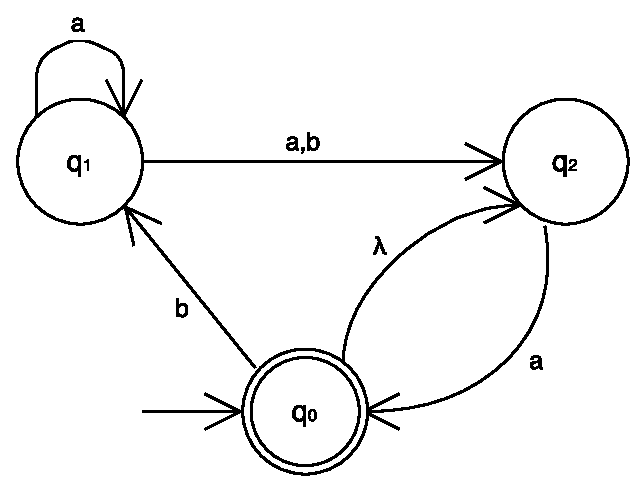
\includegraphics[scale=.45]{images/conv-l-afnd-2.pdf}}}
			   \end{center}
            \end{exampleblock}
		\end{frame}		

        \begin{frame}
			\frametitle{Conversiones}
			\framesubtitle{$\lambda$-AFND a AFD}
           
           \begin{exampleblock}{Ejercicio - Soluci\'on}
               \begin{table}
                   \begin{center}
                      {\tiny
                       \begin{tabular}{l|l|lc} 
                           \multicolumn{1}{c|}{$E(\{q_{i}\})$} & \multicolumn{1}{c}{$a$} & \multicolumn{1}{|c}{$b$} & \multicolumn{1}{|c}{$q_{i}'$} \\ \hline
                          $A=\{q_{0}\} \cup \{q_{2}\}$ & $A=\{q_{0}\} \cup \{q_{2}\}$ & $B=\{q_{1}\} \cup \O \Leftrightarrow B=\{q_{1}\} $ & $q_{0}'$ \\
                          $B=\{q_{1}\}$  & $C=\{q_{1},q_{2}\} \cup \O \Leftrightarrow C=\{q_{1},q_{2}\}$ & $D=\{q_{2}\} \cup \O \Leftrightarrow D=\{q_{2}\}$ & $q_{1}'$ \\
                          $C=\{q_{1},q_{2}\}$ & $E=\{q_{0},q_{1},q_{2}\} \cup \{q_{2}\}$ & $D=\{q_{2}\} \cup \O \Leftrightarrow D=\{q_{2}\}$ & $q_{2}'$ \\
                          $D=\{q_{2}\}$ &  $A=\{q_{0}\} \cup \{q_{2}\}$ & $---$ & $q_{3}'$ \\
                          $E=\{q_{0},q_{1},q_{2}\} \cup \{q_{2}\}$ & $E=\{q_{0},q_{1},q_{2}\} \cup \{q_{2}\}$ & $C=\{q_{1},q_{2}\}$ & $q_{4}'$ \\
                       \end{tabular}}
                   \end{center}
               \end{table}
            \end{exampleblock}
		\end{frame}	

        \begin{frame}
			\frametitle{Conversiones}
			\framesubtitle{$\lambda$-AFND a AFD}

            \begin{exampleblock}{Ejercicio - Soluci\'on (\textbf{renombrando conjunto de estados})}
               \begin{table}
                   \begin{center}
                       \begin{tabular}{lc|c|c} 
                           & $E(\{q_{i}\})$ & $a$ & $b$ \\ \hline
                            \# $\rightarrow$ & $q_{0}'$ & $q_{1}'$ & $q_{2}'$ \\
                           & $q_{1}'$ & $q_{2}'$ & $q_{3}'$ \\
                           & $q_{2}'$ & $q_{4}'$ & $q_{3}'$ \\
                           & $q_{3}'$ & $q_{1}'$ & $---$ \\
                           \# & $q_{4}'$ & $q_{4}'$ & $q_{2}'$ \\
                       \end{tabular}
                   \end{center}
               \end{table}
            \end{exampleblock}
		\end{frame}		

        \begin{frame}
			\frametitle{Conversiones}
			\framesubtitle{$\lambda$-AFND a AFD}
           
               \hspace{4cm}\huge{\textquestiondown~Aut\'omata ?}
%               \begin{center}
%			       \fbox{\fbox{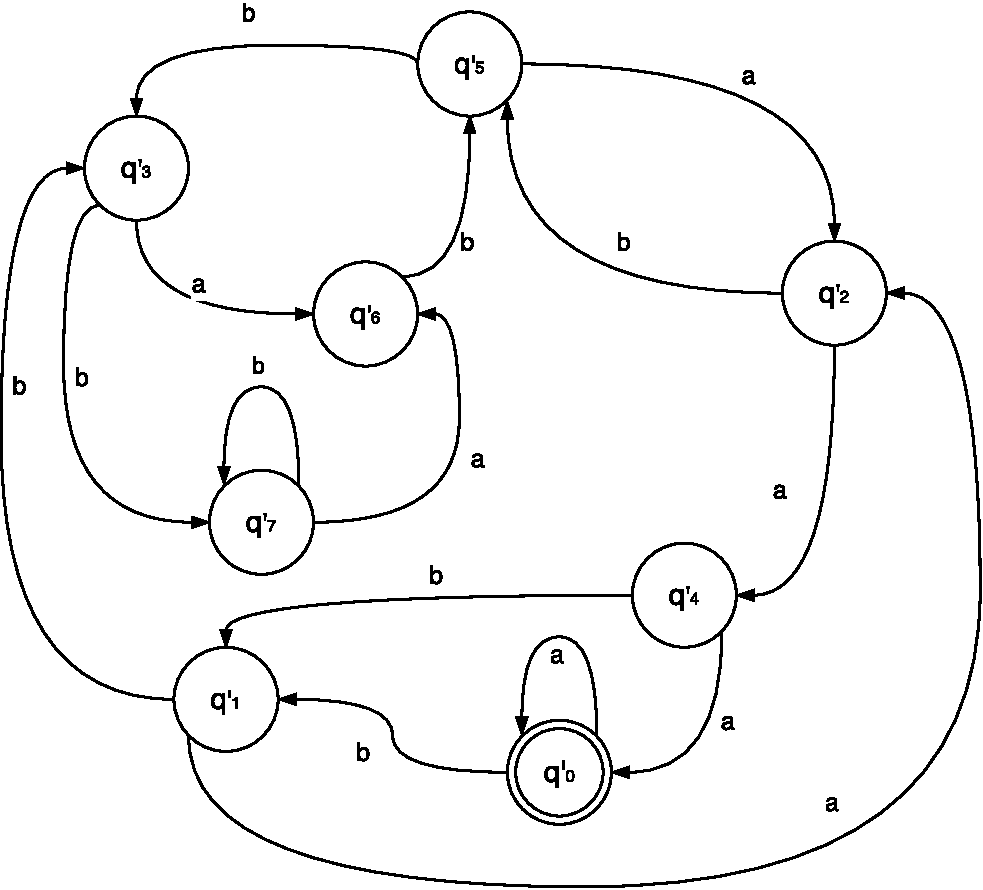
\includegraphics[scale=.4]{images/conv-afnd-2-2.pdf}}}
%			   \end{center}
		\end{frame}	

		\begin{frame}
			\frametitle{Preguntas}

			\hspace{4cm}\huge{Preguntas ?}
		
		\end{frame}
	\end{document}

\usetheme{default}
\usetheme{JuanLesPins}
\usetheme{Goettingen}
\usetheme{Szeged}
\usetheme{Warsaw}

\usecolortheme{crane}

\usefonttheme{serif}
\usefonttheme{structuresmallcapsserif}